\documentclass[11pt]{article}

%Preambel
%Umlaute und Sonderzeichen
\usepackage[T1]{fontenc}
\usepackage[utf8x]{inputenc}

%Bilder
\usepackage{graphicx}

%Ränder
\usepackage{anysize}
\marginsize{2cm}{1cm}{1cm}{1cm}

%Deutsch
\usepackage{ngerman}

%Dokument
\begin{document}
\setlength{\parindent}{0pt}

\tableofcontents
\newpage

\section{Hobbies}

\subsection{General}
Ich arbeite viel mit Tabellen und spiele gerne am Computer. 
Das Beste dan den beiden Hobbys ist, dass ich die Fähigkeit, Tabellen zu machen, gut in mein Computerpiel einbinden kann, indem ich Turniere organisiere.
Damit habe ich dann auch schon, \textit{mehr oder weniger,} Geld verdient.

\subsection{Tabellen}
Bei mir ist es wichtig, dass die Tabellen nicht nur gut funktionieren, sondern auch gut aussehen.
Natürlich sollte man die Funktionalität nicht ignorieren, in Excel bzw. Google Sheets lassen sich mit den Formeln und auch mit den Scripts sehr viel anfangen.
Trotzdem sollte man darauf aufpassen, dass die Tabellen ordentlich und übersichtlich aussehen.

\begin{figure}[hbtp]
\centering
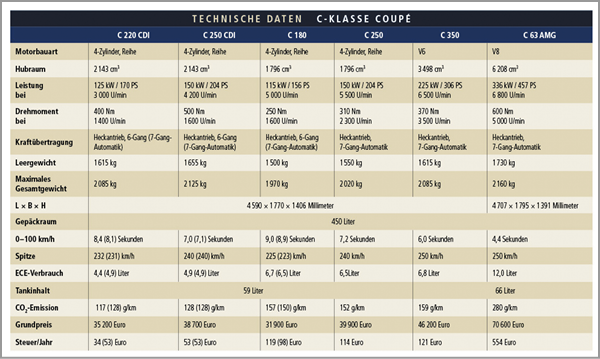
\includegraphics[width=.75\textwidth]{Bilder/ExampleSheet.png}
\caption{Beispiel Tabelle aus dem Internet}
\end{figure}


\subsubsection*{Design}
Der größte Unterschied von meinen Tabellen, verglichen zu herkömmlichen Tabellen, dass sie von Natur aus die Gridlines ausgeschaltet haben.
Dies ermöglicht mir ein moderneres Design als es ohne Gridlines möglich wäre.
Außerdem finden sich finden sichbei mir, so wie ich es immer bevorzuge, ein dunkler Hintergrund, genau genommen ein sanftes Grau.
Dort kommt dann für jede Zelle mit Inhalt ein weißer Hintergrund, als Schriftfarbe das selbe Grau wie der Haupthintergrund.
Das Grau als Schriftfarbe ist einfach sanfter auf den Augen als ein pures \#000000 Schwarz.
Dazu arbeite ich noch mit Pastell-Farben.

\newpage
\listoffigures

\end{document}